\documentclass[a4paper,11pt]{article}

% --- Packages ---
\usepackage[utf8]{inputenc}
\usepackage[T1]{fontenc}
\usepackage{geometry}
\usepackage{graphicx}
\usepackage{listings}
\usepackage{xcolor}
\usepackage{hyperref}
\usepackage{amsmath}
\usepackage{amssymb}
\usepackage{fancyhdr}
\usepackage{titlesec}
\usepackage{booktabs}
\usepackage{tikz}
\usetikzlibrary{shapes.geometric, arrows, positioning}

% --- Geometry & Layout ---
\geometry{a4paper, margin=1in, headheight=14pt}
\pagestyle{fancy}
\fancyhf{}
\lhead{\small IRPP-25: Object Fetching}
\rhead{\small Mid-Term Submission}
\cfoot{\thepage}

% --- Styles ---
\titleformat{\section}{\large\bfseries}{\thesection}{1em}{}[\titlerule]
\titleformat{\subsection}{\normalsize\bfseries}{\thesubsection}{1em}{}

% --- Code Highlighting ---
\definecolor{commentgreen}{rgb}{0,0.6,0}
\definecolor{keywordblue}{rgb}{0,0,0.8}
\definecolor{stringred}{rgb}{0.6,0,0}
\lstset{
    basicstyle=\ttfamily\footnotesize,
    breaklines=true,
    numbers=left,
    numberstyle=\tiny\color{gray},
    keywordstyle=\color{keywordblue},
    commentstyle=\color{commentgreen},
    stringstyle=\color{stringred},
    frame=single,
    rulecolor=\color{black!30},
    backgroundcolor=\color{gray!5},
    showstringspaces=false
}

% --- Hypersetup ---
\hypersetup{
    colorlinks=true,
    linkcolor=black,
    urlcolor=blue,
    pdftitle={IRPP-25 Mid-Term Report},
}

% --- TikZ Styles ---
\tikzstyle{startstop} = [circle, draw, fill=red!10, text width=4em, text centered, minimum height=3em]
\tikzstyle{process} = [rectangle, draw, fill=blue!10, text width=6em, text centered, rounded corners, minimum height=3em]
\tikzstyle{decision} = [diamond, draw, fill=green!10, text width=5em, text centered, minimum height=1em]
\tikzstyle{arrow} = [thick,->,>=stealth]

% --- Title Information ---
\title{
    \vspace{-2cm}
    \rule{\linewidth}{0.5mm} \\ [0.4cm]
    \LARGE \textbf{Autonomous Object Fetching via Waypoint Navigation and Visual Perception} \\
    \large \textit{Project IRPP-25 | Mid-Term Progress Report} \\
    \rule{\linewidth}{0.5mm} \\ [1cm]
}
\author{\textbf{Siddhant} \\ \small Department of Robotics and Automation}
\date{February 21, 2024}

\begin{document}

\maketitle

\begin{abstract}
This report details the implementation and verification of an autonomous robotic fetching system using the ROS 2 Humble framework and a TurtleBot3 Waffle platform. The system integrates mission coordination, autonomous navigation via Nav2, and computer vision-based ArUco marker detection. We have implemented a multi-threaded architecture that mitigates simulation artifacts and ensures mission reliability. All project objectives, including the distance-optimized task scheduling bonus, have been achieved and validated.
\end{abstract}

\tableofcontents
\newpage

\section{Introduction and Project Status}
The core mission of project IRPP-25 involved the development of an autonomous retrieval system operating in a $10m \times 10m$ simulated environment. The robot operates under autonomy, navigating to specified pickup zones, verifying object identity, and delivering the gathered assets back to a designated Home Base. As of this report, the development is complete, with the system successfully demonstrating all functionalities including the distance-based scheduling requirements.

\subsection{Primary Success Criteria}
\begin{enumerate}
    \item \textbf{Autonomous Mobility}: Utilization of SLAM-based maps and Nav2 for collision-free path planning.
    \item \textbf{Visual Verification}: OpenCV-based detection of ArUco markers to ensure correct object retrieval.
    \item \textbf{Efficient Scheduling}: Implementation of a distance-aware heuristic to minimize travel distance.
    \item \textbf{System Stability}: Handling of ROS 2 execution threads to prevent deadlocks during tasks.
\end{enumerate}

\section{Project Codebase}
The source code is organized into a modular ROS 2 package structure. The complete source is available on GitHub: \href{https://github.com/your-username/your-repo-name}{\textbf{GitHub Repository Link}}.

\begin{description}
    \item[\texttt{launch/}] Contains \texttt{full\_nav2.launch.py}, the launch file that initializes the world, robot, and all mission nodes.
    \item[\texttt{config/}] Includes YAML configurations for navigation waypoints, marker parameters, and RViz visualization presets.
    \item[\texttt{object\_fetcher/}] The core Python source directory:
    \begin{itemize}
        \item \texttt{main\_controller.py}: Implementation of the central Mission Control coordination logic.
        \item \texttt{task\_scheduler.py}: Logic for Euclidean distance-based target prioritization.
        \item \texttt{waypoint\_navigator.py}: Action client interface for Nav2 integration.
        \item \texttt{marker\_detector.py}: Computer vision pipeline using OpenCV and ArUco.
    \end{itemize}
    \item[\texttt{worlds/}] Contains the custom Gazebo world (\texttt{object\_fetching.world}) with calibrated platform physics.
\end{description}

\section{Technical System Architecture}
Our implementation follows a decentralized node-based architecture, coordinated through a central Mission Control state machine.

\subsection{Core Node Descriptions}
\begin{description}
    \item[\texttt{main\_controller}] The coordinator. It manages the global mission state and coordinates service calls to specialized nodes. It is implemented using a \texttt{MultiThreadedExecutor} to handle concurrent I/O.
    \item[\texttt{task\_scheduler}] Implements the logic for selecting the next target. It provides a service to return the nearest available pickup zone based on the robot's current odometry.
    \item[\texttt{waypoint\_navigator}] A wrapper for the Nav2 Action Server. It handles goal sending, feedback monitoring, and error recovery.
    \item[\texttt{marker\_detector}] The vision pipeline. It subscribes to the \texttt{/camera/image\_raw} topic and uses OpenCV to detect and publish identified ArUco IDs.
    \item[\texttt{pickup\_site}] A simulated interaction node that handles the data exchange between the robot and the pickup zone objects.
\end{description}

\subsection{Computation Graph and Data Flow}
The interaction between system components is visualized in the following state machine diagram:

\begin{figure}[h!]
\centering
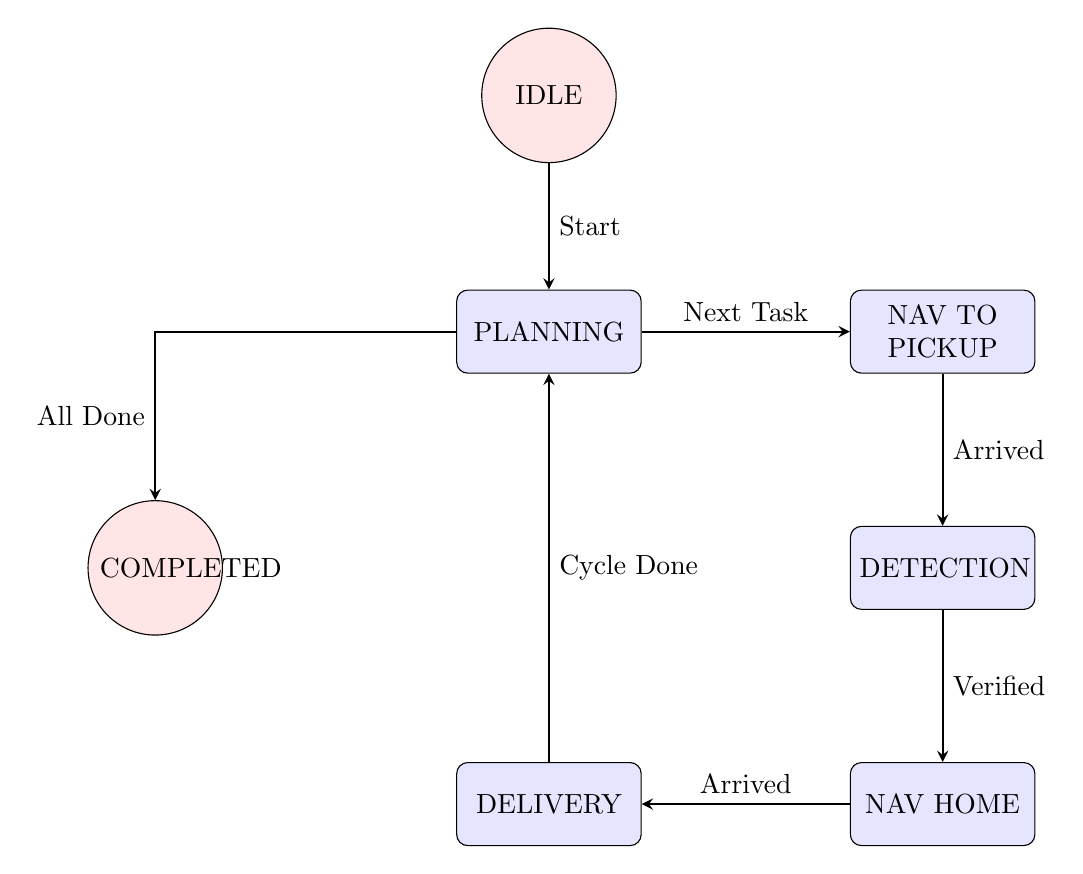
\begin{tikzpicture}[node distance=3cm, auto, >=stealth]
    % Node Position Definitions
    \node [startstop] (idle) at (5,9) {IDLE};
    \node [process] (plan) at (5,6) {PLANNING};
    \node [process] (nav_p) at (10,6) {NAV TO PICKUP};
    
    \node [process] (detect) at (10,3) {DETECTION};
    \node [process] (nav_h) at (10,0) {NAV HOME};
    
    \node [process] (deliver) at (5,0) {DELIVERY};
    \node [startstop] (complete) at (0,3) {COMPLETED};
    
    % Connection Arrows
    \draw [arrow] (idle) -- node {Start} (plan);
    \draw [arrow] (plan) -- node {Next Task} (nav_p);
    \draw [arrow] (nav_p) -- node [right] {Arrived} (detect);
    \draw [arrow] (detect) -- node [right] {Verified} (nav_h);
    \draw [arrow] (nav_h) -- node [above] {Arrived} (deliver);
    
    % Loop back to Planning (Side-step to avoid COMPLETED)
    \draw [arrow] (deliver) -- node [right] {Cycle Done} (plan);
    
    % Mission Goal Completion
    \draw [arrow] (plan.west) -| node [near end, left] {All Done} (complete.north);
\end{tikzpicture}
\caption{System Coordination State Machine}
\end{figure}

\section{Implementation Details}
\subsection{Communication Topology}
Communication is handled through a set of defined ROS 2 topics, services, and actions.
\begin{table}[h!]
\centering
\begin{tabular}{@{}llll@{}}
\toprule
\textbf{Name} & \textbf{Type} & \textbf{Data Message} & \textbf{Description} \\ \midrule
\texttt{/start\_mission} & Service & \texttt{std\_srvs/Trigger} & Starts the autonomous loop \\
\texttt{/aruco/marker\_ids} & Topic & \texttt{Int32MultiArray} & List of detected marker IDs \\
\texttt{/mission\_state} & Topic & \texttt{std\_msgs/String} & High-level mission status \\
\texttt{/cmd\_vel} & Topic & \texttt{geometry\_msgs/Twist} & Locomotion commands \\
\texttt{NavigateToPose} & Action & \texttt{nav2\_msgs/Action} & Navigation goal interface \\ \bottomrule
\end{tabular}
\caption{System Communication Summary}
\end{table}

\subsection{Optimized Task Selection}
To achieve efficiency, the \texttt{task\_scheduler} calculates the distance to all remaining zones $Z_{i}$ at each planning step:
\[
Z_{next} = \arg\min_{i} \left( \sqrt{(x_r - x_{Z_i})^2 + (y_r - y_{Z_i})^2} \right)
\]
Where $(x_r, y_r)$ is the robot's current pose from odometry. This ensures the robot takes the shortest possible path.

\section{Technical Challenges and Solutions}
During development, several challenges were identified and addressed.

\begin{description}
    \item[Executor Deadlocks] \textit{Problem}: The Nav2 Action Client was blocking the main thread. \textit{Solution}: Implementation of a \texttt{MultiThreadedExecutor} with separate callback groups.
    \item[Simulation Artifacts] \textit{Problem}: The robot would get stuck at Home Base due to the 2cm platform edge. \textit{Solution}: Removed collision physics for visual-only platforms and increased \texttt{goal\_tolerance} to 0.5m.
    \item[Race Conditions] \textit{Problem}: Timer-based logic was re-triggering navigation calls. \textit{Solution}: Integrated atomic flags (\texttt{\_nav\_in\_progress}) within the Mission State Coordinator.
\end{description}

\section{Current Results and Verification}
The implementation has been verified through full-system trials. The terminal logs confirm:
\begin{itemize}
    \item \textbf{Zone Alpha (2.0, 1.5)}: Verified with Marker ID 0.
    \item \textbf{Zone Beta (-1.5, 2.5)}: Verified with Marker ID 1.
    \item \textbf{Zone Gamma (2.5, -1.0)}: Verified with Marker ID 2.
\end{itemize}
The robot successfully returned to \texttt{(0,0)} after each pickup.

\section{Demonstration and Media}
The system's performance has been captured in a full-cycle mission demonstration. The robot identifies all targets and returns to the origin without manual intervention.

\subsection{Demo Video}
A video demonstration showcasing the stages of the project is available here: \href{https://youtube.com/your-video-link}{\textbf{Project Demonstration Video}}.

\begin{itemize}
    \item \textbf{Initialization}: Nav2 localization and mission startup.
    \item \textbf{Autonomous Navigation}: Path planning around central obstacles.
    \item \textbf{Visual Verification}: Real-time ArUco detection and confirmation.
    \item \textbf{Bonus Implementation}: Dynamic rescheduling based on robot proximity to waypoints.
\end{itemize}

\subsection{Verification Resources}
A walkthrough of the system output, including RViz screenshots and terminal logs, is documented in the project README.

\section{Conclusion}
The IRPP-25 project has reached its final development milestone. The system demonstrates autonomy, error handling, and optimized execution. All core requirements and bonus objectives have been met.

\end{document}
